% Two subsections of point_defects_report.tex: training stability, and the transformer and the
% CNN as finders. Read only when pd_table_finders.tex exists (written by
% make_report_numbers.py from the seed study and the comparison of the three networks).
\subsection{Is the training stable and repeatable?}
\label{sec:stability}

% written by make_report_numbers.py
\begin{table}[t]
\centering
\caption{Training stability. Gradient: the size (norm) of the gradient of the loss in one update, before it is cut to 1; the median and the largest value of a run. Cut: the share of updates whose gradient was larger than 1 and was scaled down. Gradient spike: a gradient more than 5 times the median of the 100 updates before it. Loss spike: a loss more than 3 times the median of the last 50 updates on the same kind of batch. Where the runs differ, the lowest and the highest are given.}
\label{tab:stability}
\footnotesize\setlength{\tabcolsep}{4pt}
\begin{tabularx}{\linewidth}{@{}>{\raggedright\arraybackslash}Xlrcccccc@{}}
\toprule
 & & & & \multicolumn{2}{c}{Gradient} & & \multicolumn{2}{c}{Spikes} \\
\cmidrule(lr){5-6}\cmidrule(l){8-9}
Finder & Start & Updates & Runs & median & largest & Cut & gradient & loss \\
\midrule
EGNN & denoiser & 2,000 & 3 & 2.0--2.5 & 38--86 & 95--96\% & 9--32 & 1--13 \\
EGNN, no class weights & denoiser & 2,000 & 2 & 0.31--0.34 & 6.2--6.7 & 1--3\% & 3--4 & 5--11 \\
EGNN & random & 2,000 & 3 & 1.4--1.5 & 4.1--5.2 & 92--93\% & 0 & 0 \\
\addlinespace
EGNN & random & 20,000 & 3 & 1.5--1.6 & 55--82 & 85--88\% & 71--131 & 14--34 \\
Transformer & random & 20,000 & 3 & 0.9--1.0 & 4.9--5.5 & 40--50\% & 0 & 0--1 \\
CNN & random & 20,000 & 3 & 1.6--1.8 & 6.3--8.1 & 85\% & 0 & 0 \\
\bottomrule
\end{tabularx}
\end{table}


Prof.\ Dabo pointed out that networks of the EGNN kind can be unstable in training. An unstable training would show in one of three ways: the loss or the gradient grows without limit and the run fails; the loss keeps jumping back up; or runs that differ only in the seed end with clearly different networks. We looked for all three. In \pd{stab-runs} training runs we recorded, at every update, the loss and the size of the gradient before it is cut (Section~\ref{sec:equations}). The gradient says how strongly one update wants to change the weights. Table~\ref{tab:stability} and Figure~\ref{fig:finders}a give the result.

\textbf{No run failed.} In none of the \pd{stab-runs} runs was a loss or a gradient ever infinite or undefined, and every run ended with a working finder.

\textbf{The results repeat.} The three runs of the reference setting find \pd{seed-ref-runs}\% of the defects (Table~\ref{tab:ablations}). This spread of \pd{abl-reference-sd} points is small beside the uncertainty that comes from the limited number of test defects, about $\pm4$ points. The three networks also find the \emph{same} defects: for \pd{seed-agree}\% of the test defects, either all three find the defect or none does. Using the three together, by averaging their probabilities, finds \pd{seed-ensemble}\%, hardly more than one alone.

\textbf{The EGNN has gradient spikes.} From time to time the gradient of the EGNN is suddenly more than five times larger than in the updates just before, in the worst case \pd{stab-max-ratio} times. When training starts from the denoiser, such spikes appear early, the first one between updates \pd{stab-ref-first} (\pd{stab-ref-gspikes} per run in 2,000 updates; largest gradient \pd{stab-ref-largest}, against a median of \pd{stab-ref-median}). From random weights there is none in the first 2,000 updates. But over 20,000 updates there are \pd{stab-egnn-gspikes} per run, the first one between updates \pd{stab-egnn-first} (Figure~\ref{fig:finders}a). At some of the spikes the loss jumps as well (\pd{stab-egnn-lspikes} times per run); training then continues as before.

\textbf{Cutting the gradient keeps the spikes harmless.} Every gradient larger than 1 is scaled down to 1 before the update. A spike can therefore change the weights no more than any other update. With this cut in place the spikes leave no trace in the results, which repeat to within a point. The cut is not a rarely used safety net. With class weights, mistakes on the rare roles count up to 32 times more, the gradients are large, and \pd{stab-egnn-cut}\% of all updates of the EGNN are cut. Without class weights the gradients are about seven times smaller (median \pd{stab-now-median}) and only \pd{stab-now-clipped}\% of the updates are cut. We did not train without the cut, so we cannot say whether the EGNN would fail without it.

\textbf{The spikes belong to the EGNN.} A transformer and a CNN, trained on the same data with the same loss, optimiser and cut (Section~\ref{sec:finders}), show no gradient spike at all in 20,000 updates; their largest gradients are \pd{stab-tr-largest} and \pd{stab-cnn-largest}. The spikes therefore come from the network, not from the data or the loss. We have not found out which part of the EGNN causes them.

In short: the EGNN trains less smoothly than the two other networks, as Prof.\ Dabo expected. With the gradient cut, its results are stable and repeat from run to run.

\subsection{Other finders: a transformer and a CNN}
\label{sec:finders}

% written by make_report_numbers.py
\begin{table}[t]
\centering
\caption{Three kinds of network as finder: defects found (\%) on the real test defects. The first three rows were trained in exactly the same way, from random starting weights; each is the mean of three runs that differ in the random seed, with the spread between the runs after the $\pm$. The two rows below them are the EGNN that starts from the denoiser (one run each). Last row: the six transformer and CNN runs used together, by averaging their probabilities. Size in millions of parameters.}
\label{tab:finders}
\footnotesize\setlength{\tabcolsep}{3.2pt}
\begin{tabularx}{\linewidth}{@{}>{\raggedright\arraybackslash}Xlrccccccl@{}}
\toprule
Finder & Start & Updates & Runs & Size & Vacancy & Interst. & Antisite & Frenkel & All \\
\midrule
Transformer & random & 20,000 & 3 & 0.58 & 67.2 & 48.3 & 54.2 & 42.0 & 53.6 $\pm$ 0.3 \\
CNN & random & 20,000 & 3 & 0.50 & 69.7 & 51.2 & 52.8 & 38.4 & 54.0 $\pm$ 0.5 \\
\addlinespace
EGNN & random & 20,000 & 3 & 0.52 & 63.2 & 29.7 & 44.0 & 35.1 & 43.5 $\pm$ 0.5 \\
EGNN & denoiser & 20,000 & 1 & 0.52 & 67.0 & 47.5 & 46.5 & 36.7 & 50.3 \\
EGNN, main finder & denoiser & 60,000 & 1 & 0.52 & 69.5 & 50.0 & 49.0 & 45.3 & 54.0 \\
\addlinespace
Transformer + CNN, all six runs & random & 20,000 & 6 & -- & 70.0 & 49.5 & 56.0 & 41.3 & 55.1 \\
\bottomrule
\end{tabularx}
\end{table}


\begin{figure}[t]
\centering
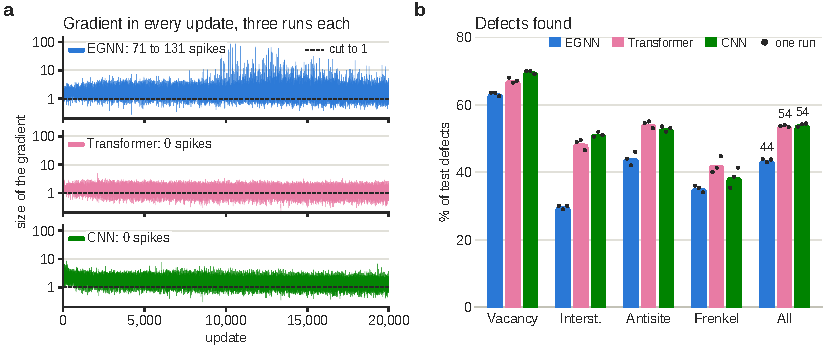
\includegraphics[width=\linewidth]{figures/pd_fig5_finders.pdf}
\caption{Three kinds of network as finder, trained in the same way from random starting weights. (a)~The size of the gradient at every one of the 20,000 updates, three runs per network, before it is cut to 1 (dashed line). Note the scale: each step up is ten times larger. The spike counts are the lowest and highest of the three runs. (b)~Defects found on the real test defects. Bars: mean of three runs; dots: the single runs. All values are in Tables~\ref{tab:stability} and~\ref{tab:finders}.}
\label{fig:finders}
\end{figure}

Is a graph network the right kind of network for finding defects? We built the finder from two other kinds of network as well (Section~\ref{sec:baselines}): a transformer, in which every atom looks at all other atoms at once, and a CNN, which looks at the glass as a picture. To compare the kind of network and nothing else, all three were trained in exactly the same way: from random starting weights, on the same data, with the same loss, class weights and optimiser, for 20,000 updates, three runs each. The EGNN trained in this way is the \emph{control}. All three have about half a million parameters.

\textbf{Both find more than the EGNN.} The transformer finds \pd{fin-tr-all}\% of all test defects and the CNN \pd{fin-cnn-all}\%; the EGNN finds \pd{fin-egnn-all}\% (Table~\ref{tab:finders}, Figure~\ref{fig:finders}b). The runs of one network differ by half a point or less, so a lead of ten points is far outside chance. Compared on the same defects, run by run, each of the two is ahead of the control in all three runs (\pd{fin-p-tr}): it finds \pd{fin-only-tr} (transformer) or \pd{fin-only-cnn} (CNN) defects that the control misses and misses about 40 that the control finds. Most of the lead comes from interstitials (\pd{fin-tr-interstitial}\% and \pd{fin-cnn-interstitial}\% against \pd{fin-egnn-interstitial}\%) and antisites (\pd{fin-tr-antisite}\% and \pd{fin-cnn-antisite}\% against \pd{fin-egnn-antisite}\%). For vacancies and Frenkel pairs the lead is 3 to 7 points.

\textbf{The transformer and the CNN are equal.} Compared with each other on the same defects, neither is ahead (\pd{fin-p-tr-cnn} in the three runs). The CNN finds a few more vacancies and interstitials and the transformer a few more Frenkel pairs, but differences this small are common when two methods are equally good.

\textbf{Against the finder of the main results.} The finder of the main results is an EGNN that starts from the denoiser and was trained for 60,000 updates. It finds \pd{fin-main-all}\% of the test defects. The transformer and the CNN find as many from random starting weights and with a third of the updates. Starting from the denoiser still helps the EGNN after 20,000 updates (\pd{fin-pre-all}\% against \pd{fin-egnn-all}\% from random weights, \pd{fin-p-pre}; one run), but the kind of network makes the larger difference.

\textbf{The networks agree on which defects are hard.} With the same seed, \pd{fin-by-all}\% of the defects are found by all three networks and \pd{fin-by-none}\% by none of them. Using the transformer and the CNN together, by averaging the probabilities of all six runs, finds \pd{fin-six-all}\% {\small[\pd{fin-six-lo}, \pd{fin-six-hi}]}, which is not significantly more than the best single run (\pd{fin-six-p}). The three kinds of network therefore mostly succeed and fail on the same defects, and more than a third of the defects are hidden from all of them. This suggests that yet another kind of network would not find many of them either.

\textbf{Symmetry.} The EGNN and the transformer use only the distances between atoms. Their answer cannot change when the glass is shifted, turned or its atoms renumbered, and a direct test confirms it: the flagged atom stays the same in 100\% of the test glasses. A picture is made of pixels, and the CNN does not have this property by construction. Quarter turns and mirror images leave its answer unchanged, because we average over them. But when the glass is shifted by a random distance, the CNN flags a different atom in \pd{fin-cnn-noshift}\% of the glasses. For a physical method this is a flaw: the answer should not depend on where the edge of the box happens to lie.

\textbf{Cost.} One run takes \pd{fin-tr-hours} hours for the transformer and the CNN and \pd{fin-egnn-hours} hours for the EGNN, on one T4 GPU. For larger systems the order would change. The transformer compares every atom with every other, so its cost grows with the square of the number of atoms; the cost of the EGNN and of the CNN grows in proportion to the size of the system.

\textbf{What this does and does not show.} We can only suggest why the EGNN is behind. Reach is not the reason: four EGNN layers reach $10\sigma$, more than half of the box, so all three networks can see the whole glass. They differ in how they combine what they see. The EGNN builds its picture of the surroundings from sums of messages between neighbours, layer by layer. The transformer weighs every pair of atoms directly in each layer, and the CNN sees empty and crowded places as dark and bright areas of a picture. A missing or an extra atom may be easier to read in these two ways. We have not tested this explanation. Three further limits apply. The comparison is at one length of training. Only finding was compared: the repair was not repeated with the new finders. And the transformer had two small advantages, 10\% more parameters and a learning rate that rises gradually over the first 1,000 updates; the CNN had neither and did equally well.
